\documentclass[preprint2,numberedappendix,tighten,twocolappendix]{aastex6}  % USE THIS TO MAKE BIB, THEN FORMAT USING EMULATEAPJ
%\documentclass[twocolumn,apj,numberedappendix]{emulateapj}
\shorttitle{Adding Sensitivity to 21cm Inteferometric Probes of Reionization}
\shortauthors{Zhang\&Parsons}
\usepackage{float}
\usepackage{amsmath}
\usepackage{graphicx}
\usepackage[figuresright]{rotating}
%\usepackage{rotating}
\usepackage{natbib}
%\usepackage{pdflscape}
%\usepackage{lscape}
\usepackage{ctable}
\citestyle{aa}
\renewcommand\[{\begin{equation}}
\renewcommand\]{\end{equation}}


\begin{document}

\title{Adding Sensitivity to 21cm Inteferometric Probes of Reionization by Optimizing Choice of Baselines}

%\maketitle
\author{
Yunfan Gerry Zhang \altaffilmark{1},
Aaron R. Parsons\altaffilmark{1}\altaffilmark{2}
}

\altaffiltext{1}{Astronomy Dept., U. California, Berkeley, CA}
\altaffiltext{2}{Radio Astronomy Lab., U. California, Berkeley, CA}

\begin{abstract}
We introduce an accurate method to extract additional sensitivity from data of redundant radio arrays. Our method efficiently finds optimal baselines to cross correlate, including baselines that are slightly different in length and orientation. 
Using the latest and final 128-element version of Precision Array for Probing the Epoch of Reionization (PAPER-128), as well as the planned 37, 128, 240 and 350 element versions of the Hydrogen Epoch of Reionization Array (HERA) now under development, we illustrate how our method applies to different array configurations and predict the sensitivity improvements of including each baseline pairs. The extremely natural and simple implementation of this method
would increase the sensitivity of PAPER-128 by about to $10\%$, and increase the out-rigger imaging sensitivity of HERA-350 by a factor of 2. 
\end{abstract}

\section{Introduction}

The epoch of reionization, or cosmic dawn represents the last key
stage of the universe's early evolution. Study of this event stands at
the intersection of cosmology and astrophysics. Understanding this
event is important not only because it is a scientific goal
of its own, but also because it can provide crucial information
to fundamental physics of inflation, neutrino mass and phenomenology
of the first stars and galaxies (e.g. \cite{LiuOpticalDepth}). 

Arguably the most promising observational probe of the epoch of reionization
comes from measurement of the ``spin-flip'' transition of neutral
hydrogen of characteristic wavelength 21cm \cite{Furlanetto2006181,PritchardLoeb}.
While probes such as quasar spectra rely on emission and scattering
of free electrons, and are thus limited to the lower redshifts towards the end of reionization, the 21cm line directly probes the
abundance and distribution of neutral hydrogen, and thus would potentially
shed light on all stages of reionization. Radio interferometry efforts
to measure the 21cm power spectrum has been a top priority in recent years of astronomy.
Current generation instruments include the Precision Array for Probing
the Epoch of Reionization (PAPER) \cite{Ali2015,paper32}, Murchison
Widefield Array (MWA) \cite{MWA}, Low Frequency Array (LOFAR) \cite{LOFAR}. Next generation instruments such as the Hydrogen Epoch of Reionization
Array (HERA) (e.g. \cite{HERA,HERAconfiguration,HERABEAM1,HERADISH2})
and the Square Kilometer Array Low (SKA low) (e.g. \cite{SKA1}) are
in planning and construction. 

One of the main challenges of interferometric observations of cosmic
21cm line is foreground contamination. Both sources within our
galaxy, and to a lesser distant sources outside of our galaxy emit
radio contaminations (via for example synchrotron processes) up to five orders of magnitude stronger than the
reionization signal. There are two common methods to deal with the
foreground contamination. In the first, sometimes called the foreground
removal technique, individual sources are identified and removed in the image domain.
The other technique, commonly referred to as 'foreground avoidance',
makes use of the fact that most common foreground contaminations have a smooth
spectrum, and thus is constrained to a Fourier domain ``foreground
wedge'' \cite{wedge1,wedge2}. Thus contamination can be avoided
by restricting our observation to ``outside the wedge'', where the data is currently noise dominated. The main
challenge of using the avoidance technique is thus the sensitivity, or
the signal to noise ratio. This is the motivation for the design of
the maximum redundancy arrays such as PAPER and HERA. Traditional
imaging arrays are designed to image localized bright sources and thus favor non-redundant patterns for uv coverage. The redundant arrays on the other hand
focus on high-sensitivity measurements of the same Fourier mode
with many tightly packed antennas at equal spacing. Since baselines
of the same length and orientation measure the same Fourier modes
on the sky, a maximum redundancy array is able to increase the
signal to noise ratio by averaging over measurements of the same baseline.
\cite{Ali2015} provides the newest upper limit to the power spectrum
measurements with the 64-element version of PAPER(henceforth referred to as PAPER-64). From some models we roughly expect
that the sensitivity required for detection is a factor of 10 away.
This paper explores a new technique to add sensitivity to the analysis
of redundant arrays, by making use of the earth's rotation. This technique
can be applied to redundant arrays such as PAPER and HERA to increase
the sensitivity by up to a factor of [1.5]. 

The earth's rotation causes the baselines to pick up different modes of the sky with time. 
This effect is used extensively to improve uv coverage in imaging with minimum redundancy arrays. In
a maximally redundant array, baselines that are slightly different
rotate into each other at a time delay. Here we present a method to
improve the sensitivity of the maximum redundancy arrays by including
the uv redundancy of different baselines at a time lag. Recently the authors of \cite{wterm} proposed an algorithmic search approach to extract information from all near-equivalent baselines. We here present a simple and elegant theoretical formalism that in addition allows us to identify good baselines to cross-correlate and predict the weight of sensitivity with speed and accuracy. 

Baselines of the same length and orientation are traditionally called
``redundant baselines'', because they measure the same Fourier mode
in the sky. In order to eliminate confusion and ambiguity, we shall
introduce slightly different terminology. We'll call baselines that
are the same length and orientation ``equivalent baselines'', inspired
by the mathematical notion of equivalency classes. Two equivalent
baselines will be redundant with each other simultaneously at all
times. Non-equivalent baselines can also be partially redundant if their
respected time series is shifted with respect to one another by a
certain delay. In other words, one baseline can be ``rotated into''
another. We call these ``near-equivalent baselines''. It is our
goal to a) identify the near-equivalent baselines that give good
redundancy, b) to find the optimal time offset for a given pair of baselines, and
c) to quantify the sensitivity improvement associated with cross multiplying
such a pair of near-equivalent baselines. In section
2 we explain the theoretical basis for this cross multiplication.
In section 3 we present numerical tests of
this technique as well as the expected sensitivity improvement
with this method for HERA and PAPER-128 and with section 4 we conclude. 


\section{Method}

\subsection{Rough Idea}

\begin{figure}[H]
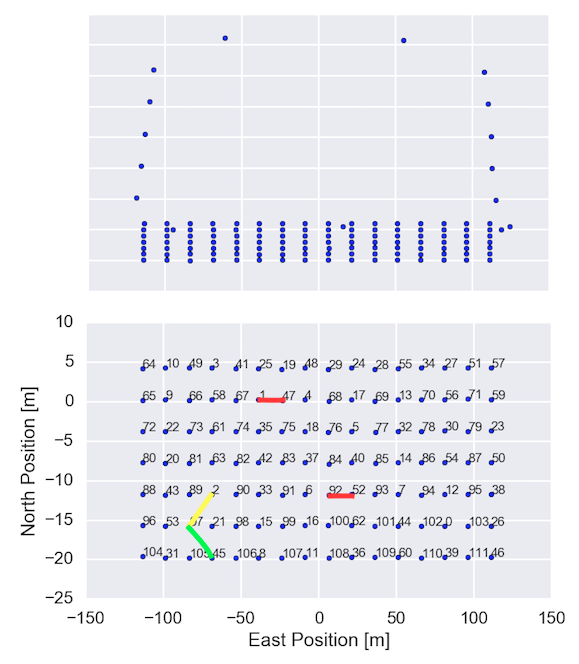
\includegraphics[width=\linewidth]{antpos128}

\caption{The PAPER-128 layout. Each blue dot corresponds to the location of
an antenna. Top panel shows the antenna positions drawn to scale,
bottom panel show the antenna labels and distances, excluding the outlier
antennas.\label{fig:AntPos}
The numbering of the antennas the bottom panel are original labels
during instrument assembly and does not bear significant
meaning. Baselines corresponding to the same separations are called
equivalent. In the bottom panel, the two baselines labeled with the
red arrow are equivalent, with separation denoted by sep1,0, for the
antennas are separated by 1 unit east and 0 unit north. Similarly,
the baselines labeled with the yellow and green arrows are examples
of sep1,1 and sep1,-1, respectively. Note sep1,0 and sep-1,0 for example
are the same baselines and should not be counted twice.}

\end{figure}

We shall use the 128-element PAPER array to demonstrate. 
The PAPER array is located in the Karoo desert in South Africa (30:43:17.5
S, 21:25:41.8 E). The layout pattern with antenna labels are show
in Fig. \ref{fig:AntPos}. We see the antenna spacing in North-South
directions are comparatively close (4m), so that baselines such as
0\_44 and 0\_7 are very close to equivalent. In the bottom panel,
the two baselines labeled with the red arrow are equivalent, with
separation denoted by sep1,0, for the antennas are separated by 1
unit east and 0 unit north. Similarly, the baselines labeled with
the yellow and green arrows are examples of sep1,1 and sep1,-1, respectively.
Note sep1,0 and sep-1,0 for example are the same baselines and should
not be counted twice. Antennas in purely north-south baselines
are close enough to induce cross talks, and hence are not suitable
for use. The original PAPER-64 analysis (\cite{Ali2015}) used three classes of baselines, here
equivalent to 
sep2,0, sep2,1 and sep2,-1 \cite{Ali2015} of PAPER-128. There each of these classes
of baselines are cross multiplied to itself. We shall see that in addition these
baseline classes can be cross multiplied with a time offset.


Given a point source on the sky, each baseline maps the
source to a point in uv plane. As the earth rotates with respect to
the source, the point traces out tracks in the uv-plane. 
We show in Fig. \ref{fig:Tracks} uv tracks of PAPER-128 over 4.8 hours, at 0.15GHz, for a source that passes through zenith. 


\begin{figure}[H]
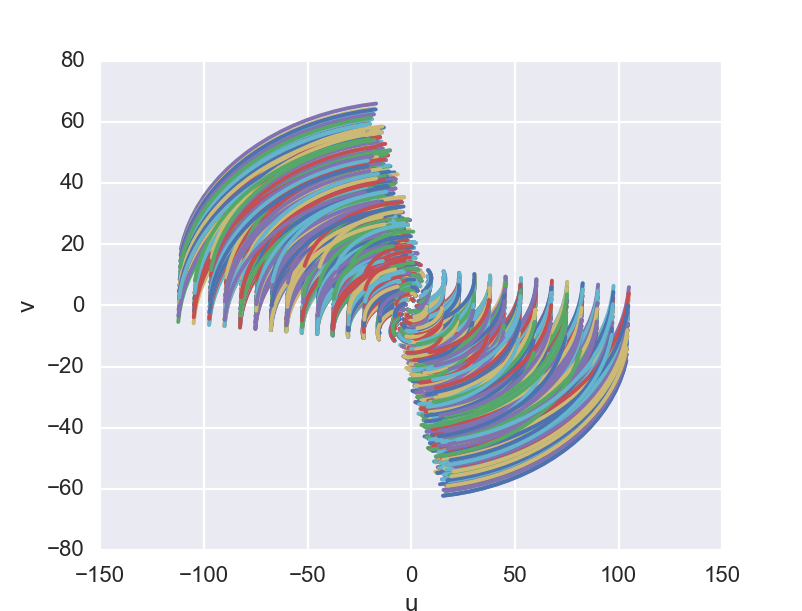
\includegraphics[width=\linewidth]{tracks128}
\caption{Tracks of PAPER-128 (grid only, excluding outliers) for a hypothetical source that passes through zenith.
These tracks are traced out over 0.2 sidereal days, or roughly 4.8
hours. Color represents different baselines. Frequency is $\nu=0.15\text{GHz}$.
As the earth rotates, tracks are traced out counterclockwise. \label{fig:Tracks}}
\end{figure}

Roughly speaking, we can identify
redundancy of near-equivalent baselines as crossings
of the uv tracks. Although this is a valid quick method to identify some baselines to cross-multiply, we find
that it is not accurate enough for time offset determination. The reason is that UV tracks are traces of a point source, which though adequate for traditional narrow beam imaging, are not applicable for wide-beam receivers like that of PAPER.
Here the uv-imprint of the sky for a given baseline and frequency is really a cloud that's the track convolved with the appropriate point-spread function. To accurately
constrain redundancy, a more rigorous treatment is thus required. 
We show sample beams of HERA and PAPER antennas in Fig.\ref{fig:Beam} for reference. 

\begin{figure}[H]
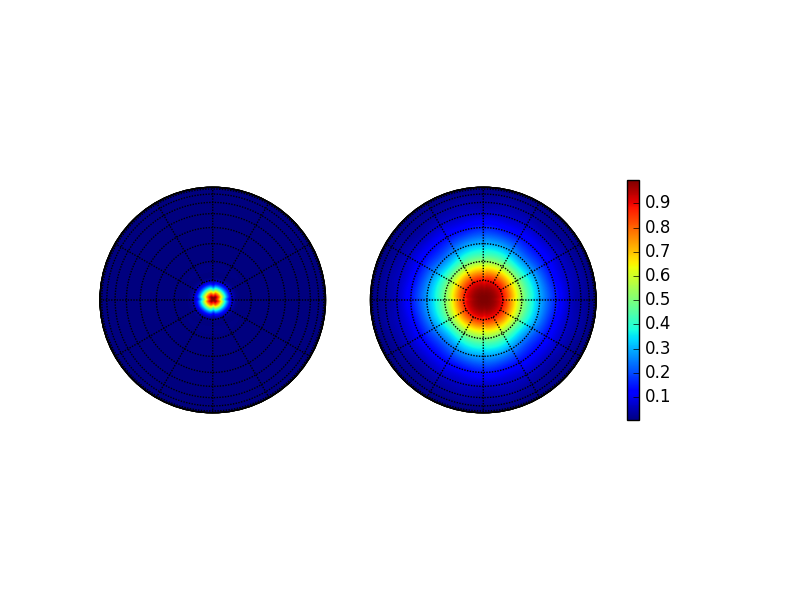
\includegraphics[width=1.2\linewidth]{Beams}

\caption{Sample beam response of HERA (left) and PAPER (right) antennas, both
for frequency of $\nu=150\text{MHz}$ and Stokes $I$ polarization. Notice $A$ in this paper is a ``baseline's beam'', equivalent to squares of the antenna beams shown here. The circles centered around zenith (center of beam) here are
spaced 10 degrees apart. The finite size of the beams limits the accuracy of the uv track-crossing as a method of redundancy search. \label{fig:Beam}}
\end{figure}



\subsection{Formalism}
Below we shall derive theoretical expectations of cross multiplications
of two near-equivalent baselines. More precisely we shall relate
the product of visibilities of two different baselines to the power spectrum. 


We take the visibility as commonly defined in the literature (e.g.
\cite{first-paper}): 
\begin{equation}
\begin{aligned}V_{\nu}(\boldsymbol{b}) & =\int d\Omega A_{\nu}(\hat{\boldsymbol{s}})\phi(\nu)I_{\nu}(\hat{\boldsymbol{s}})\exp\left[-2\pi i\frac{\nu}{c}\boldsymbol{b}\cdot\hat{\boldsymbol{s}}\right],\\
 & \approx\frac{2k_{B}}{\lambda^{2}}\int d\Omega A_{\nu}(\hat{\boldsymbol{s}})\phi(\nu)T(\hat{\boldsymbol{s}})\exp\left[-2\pi i\frac{\nu}{c}\boldsymbol{b}\cdot\hat{\boldsymbol{s}}\right],
\end{aligned}
\label{eq:Vis1}
\end{equation}
Here $\lambda$ is a mean wavelength, $\boldsymbol{b}$ is the baseline
length, $\hat{\boldsymbol{s}}$ and $\Omega$ are a direction in the
sky and its corresponding solid angle. $A_{\nu}$ is the (frequency
dependent) beam, and $I$ is the specific intensity, which has been
related to $T$, the brightness temperature in the Rayleigh-Jeans
limit. Note that $A$ here is the baseline beam, i.e. product of two antenna beams, examples of which are shown in Fig.\ref{fig:Beam}. $\phi(\nu)$ is the frequency bandpass profile. In practice,
power spectrum measurements are typically taken from a few ten MHz centered around the corresponding redshift of interest (e.g. 150 MHz for z=9.5). 

We define the delay transformed visibility \cite{delay-transform}:
\small
\begin{equation}
\begin{aligned}V(\boldsymbol{b},\tau) & =\int d\nu V_{\nu}(\boldsymbol{b})\phi(\nu)\exp\left[-2\pi i\nu\tau\right],\\
 & =\frac{2k_{B}}{\lambda^{2}}\int d\Omega d\nu A(\hat{\boldsymbol{s}},\nu)\phi(\nu)T(\hat{\boldsymbol{s}},\nu)\exp\left[-2\pi i\nu\left(\frac{\boldsymbol{b}\cdot\hat{\boldsymbol{s}}}{c}+\tau\right)\right]
\end{aligned}
.\label{eq:Vb1}
\end{equation}
\normalsize


Eq. \eqref{eq:Vb1} expresses the delay-transformed visibility as
an integral over observation coordinates $\hat{\boldsymbol{s}}$ and $\nu$. Ultimately,
we would like to relate the data, collected with coordinates $\hat{\boldsymbol{s}}$
and $\nu$, to the power spectrum, written with cosmological coordinates
$\boldsymbol{r}$ and $\boldsymbol{k}$. We start by noticing that
{[}Gerry: change all r and k into bold{]} 
\[
\begin{aligned}r & =\frac{c}{H_{0}}\int_{0}^{z}\frac{dz'}{E(z')},\\
 & \approx\frac{c}{H_{0}}\int_{0}^{z_{0}}\frac{dz'}{E(z')}-\frac{c(1+z)^{2}}{\nu_{21}H_{0}E(z)}\left(\nu-\nu_{0}\right),\\
 & \equiv D_{c}-Y\Delta\nu,
\end{aligned}
\]
where $\nu_{21}=1420MHz$ is the 21cm transition rest frequency, $\nu_{0}$
a reference central frequency with corresponding redshift $z_{0}$,
and 
\[
E(z)=\sqrt{\Omega_{m}(1+z)^{3}+\Omega_{\Lambda}}.
\]
Inverting for $\nu$:
\begin{equation}
\nu=\frac{D_{c}-r}{Y}+\nu_{21}.\label{eq:nur}
\end{equation}
Thus $d\nu=-dr/Y$ and $d^{3}r=-X^{2}Yd\Omega d\nu$. 

We can thus rewrite the delayed transformed visibility as 
\small
\[
\begin{aligned}V(\boldsymbol{b},\tau) & =\frac{1}{X^{2}Y}\int_{H}d^{3}rA(\boldsymbol{r})\phi(r)I(\boldsymbol{r})\exp\left[-2\pi i\left(\frac{\boldsymbol{b}}{c}\cdot\hat{\boldsymbol{r}}+\tau\right)\nu_{r}\right]\end{aligned}.
\]
\normalsize
Here $(r_{x},r_{y},r_{z})=(X\hat{\boldsymbol{s}}_{x},X\hat{\boldsymbol{s}}_{y},Y\nu)$, and
$(Xk_{x},Xk_{y},Yk_{z})=\frac{2\pi}{c}(b_{x},b_{y},\tau)$ relate
the cosmological coordinates $r$ and $k$ to the measured coordinates.
We have written $\nu_{r}$ to remind us that $\nu$ and $r$ are related
by Eq. \eqref{eq:nur}. The beam reception pattern $A$ is dimensionless,
normalized to 1 at its peak (zenith), and we assume it to be the same
for all baselines. 

With a time offset, the beam pattern has moved relative to the sky.
Here we choose to fix the sky, and denote the rotated coordinates
of the beam pattern with the operator $\Gamma$. With implicit bounds
of integrals from $-\infty$ to $\infty$, we have:
\begin{widetext}
\begin{equation}
\begin{aligned} & \langle V^{*}(\boldsymbol{b},\tau)V(\boldsymbol{b'},\tau')\rangle\\
 & =\left(\frac{2k_{B}}{X^{2}Y\lambda^{2}}\right)^{2}\int d^{3}rd^{3}r'\left(\langle T^{*}(\boldsymbol{r})T(\boldsymbol{r'})\rangle\right)A^{*}(\boldsymbol{r})A(\Gamma r')\Phi_{b,\tau}(\boldsymbol{r},\Gamma r'),\\
 & =\left(\frac{2k_{B}}{X^{2}Y\lambda^{2}}\right)^{2}\int d^{3}rd^{3}r'\left(\int\frac{d^{3}\kappa}{(2\pi)^{3}}\frac{d^{3}\kappa'}{(2\pi)^{3}}\langle T^{*}(\boldsymbol{\kappa})T(\boldsymbol{\kappa'})\rangle e^{-i(\boldsymbol{\kappa}\cdot \boldsymbol{r}-\boldsymbol{\kappa'}\cdot\boldsymbol{r'})}\right)A^{*}(\boldsymbol{r})A(\Gamma r')\Phi_{b,\tau}(\boldsymbol{r},\Gamma r'),\\
 & =\left(\frac{2k_{B}}{X^{2}Y\lambda^{2}}\right)^{2}\int d^{3}rd^{3}r'\left(\int\frac{d^{3}\kappa}{(2\pi)^{3}}P(\kappa)e^{-i\boldsymbol{\kappa}\cdot(\boldsymbol{r}-\boldsymbol{r'})}\right)A^{*}(\boldsymbol{r})A(\Gamma r')\Phi_{b,\tau}(\boldsymbol{r},\Gamma r'),\\
 & =\left(\frac{2k_{B}}{X^{2}Y\lambda^{2}}\right)^{2}\int d^{3}rd^{3}r'\xi(\boldsymbol{r}-\boldsymbol{r'})A^{*}(\boldsymbol{r})A(\Gamma r')\Phi_{b,\tau}(\boldsymbol{r},\Gamma r'),\\
 & \approx\left(\frac{2k_{B}}{X^{2}Y\lambda^{2}}\right)^{2}P(k_{b,\tau})\int d^{3}rd^{3}r'\delta_{D}^{(3)}(\boldsymbol{r}-\boldsymbol{r'})A^{*}(\boldsymbol{r})A(\Gamma r')\Phi_{b,\tau}(\boldsymbol{r},\Gamma r'),\\
 & =\left(\frac{2k_{B}}{X^{2}Y\lambda^{2}}\right)^{2}P(k_{b,\tau})\int d^{3}r|A^{*}(\boldsymbol{r})A(\Gamma r)||\phi(\nu_{r})|^{2}\exp\left[-i2\pi\nu_{r}\left(\hat{\boldsymbol{r}}\cdot\frac{\boldsymbol{b}}{c}-\hat{\Gamma r}\cdot\frac{\boldsymbol{b'}}{c}\right)\right],\\
 & =\left(\frac{2k_{B}}{\lambda^{2}}\right)^{2}P(k_{b,\tau})\int\frac{d\Omega d\nu}{X^{2}Y}|A^{*}(\hat{\boldsymbol{s}},\nu)A(\hat{\Gamma s},\nu)||\phi(\nu)|^{2}\exp\left[-i2\pi\nu\left(\hat{\boldsymbol{s}}\cdot\frac{\boldsymbol{b}}{c}-\hat{\Gamma s}\cdot\frac{\boldsymbol{b'}}{c}\right)\right],
\end{aligned}
\label{eq:main}
\end{equation}

where in transition from cosmological coordinates back to observing coordinates we have written $\hat{\boldsymbol{r}}\equiv\hat{\boldsymbol{s}}$, and 
\begin{equation}
\Phi_{b,\tau}(\boldsymbol{r},\Gamma r')=|{\phi^{*}}(\ensuremath{\nu_{r}})\phi(\nu_{r'})|\exp\left[-i\frac{2\pi}{c}\left(\boldsymbol{b}\cdot\nu_{r}\hat{\boldsymbol{r}}-\boldsymbol{b'}\cdot\nu_{r'}\Gamma\hat{r'}\right)\right]\exp\left[-i2\pi\tau\left(\nu_{r}-\nu_{r'}\right)\right].
\end{equation}
\end{widetext}
The second to third line of Eq.(\ref{eq:main}) follows from assumption of Gaussian random
sky, and the third to fourth line follows from the assumption that
the 3D power spectrum varies negligibly over the region of interest
so that $\hat{P_{21}}(k+k_{2})\approx\hat{P_{21}}(k)$. Since $\Gamma$
is a sky rotation, it doesn't affect $\nu$, hence we have taken $\nu_{r}$
outside the parenthesis. Notice that the phase factor $\exp\left[-i2\pi\tau\left(\nu-\nu'\right)\right]$
drops out in the end. This means that correlation is peaked at the same time-offset for all delay channels. 

Finally, since the beam pattern and bandwidth are given in $\hat{\boldsymbol{s}}$
and $\nu$, we convert the integral back to these coordinates to get
the general relation between the delay-transformed visibilities and
the power spectrum:

\begin{equation}
\begin{aligned} & \langle V^{*}(\boldsymbol{b},\tau)V(\boldsymbol{b'},\tau')\rangle\\
 & =\left(\frac{2k_{B}}{\lambda^{2}}\right)^{2}P(k_{b,\tau})\int\frac{d\Omega d\nu}{X^{2}Y}|A^{*}(\hat{\boldsymbol{s}},\nu)A(\hat{\Gamma s},\nu)||\phi(\nu)|^{2}\\
 & \qquad \qquad \qquad \qquad \exp\left[-i2\pi\nu\left(\hat{\boldsymbol{s}}\cdot\frac{\boldsymbol{b}}{c}-\hat{\Gamma s}\cdot\frac{\boldsymbol{b'}}{c}\right)\right].\end{aligned}
\label{eq:final}
\end{equation}

In other words the power spectrum estimate from visibilities of a baseline pair is given by 
\begin{equation}
 P(k_{b,\tau}) = \left(\frac{\lambda^{2}}{2k_{B}}\right)^{2} \frac{\langle V^{*}(\boldsymbol{b},\tau)V(\boldsymbol{b'},\tau')\rangle}{\Theta}, 
 \label{eq:opp}
\end{equation}
where the weight
\begin{equation}
\Theta =\int\frac{d\Omega d\nu}{X^{2}Y}|A^{*}(\hat{\boldsymbol{s}},\nu)A(\hat{\Gamma s},\nu)||\phi(\nu)|^{2} e^{-2\pi i\nu\left(\hat{\boldsymbol{s}}\cdot\frac{\boldsymbol{b}}{c}-\hat{\Gamma s}\cdot\frac{\boldsymbol{b'}}{c}\right)}. 
\label{eq:Theta}
\end{equation}



So roughly speaking the cross multiplications of visibilities at a time delay
in uv-space is proportional to the power spectrum times the Fourier
transform of the cross multiplied beam pattern. We can then in principle
combine information from different baseline pairs if we correct for
the phase and normalization. As a check, when applied to equivalent baselines,
$\boldsymbol{b}=\boldsymbol{b'}$, $\hat{\boldsymbol{s}}=\hat{\Gamma s}$, and Eq.(\ref{eq:final}) reduces to Eq.(B9) of \cite{paper32}. 

If this result is robust, then we can achieve all our goals stated in the introduction, i.e. to identify 
candidate baseline pairs, to find the optimal time offset, and to quantify the sensibility, by computing the weight $\Theta$ from
Eq.(\ref{eq:Theta}) for various time offsets. Thus we shall first test its robustness numerically.

\subsection{Rephasing \label{sec:rephs}}
Before we discuss tests, there is one subtlety when applying Eq. \ref{eq:final}. The optimal time offset is given by the $\Gamma$ that maximizes the absolute value of the weight $\Theta$. However, $\Theta$ is in general complex. First integrating over the spatial dimension $\Omega$, we see the phase term at peak time-offset is inevitably frequency dependent. This frequency dependence of the phase would lead to destructive interference when we integrate over frequency.

The physical origin of this frequency dependent phase lies the two visibilities having different phase centers. By default the two visibilities are both phased to zenith at the same time. When they are cross-correlated, they must be rephased to the account for the movement of the zenith. Thus in practice we must rephase the visibilities before delay transform. 


In Fig.\ref{fig:freqdiff} we compare two channels 0.16 GHz and 0.17 GHz.  Top panels show the equivalent baseline pairs sep1,0 against itself, and bottom panels show sep1,0 against sep1,1. The left two panels have zero rephasing, and the right two are rephased to a time offset of 0.055 sidereal days, the optimal time offset for the given baseline pair. We see that in bottom left panel, although the magnitude, drawn by the wide curves match up for the two frequencies, the phases do not. This means the wider the frequency profile, the more destructive the interference, and lower the sensitivity contribution. In the rephased case, the phases of the near-equivalent case match up and can be added without compromising sensitivity. We should thus rephase the data separately for each set of baseline pairs. 

\begin{figure}[H]
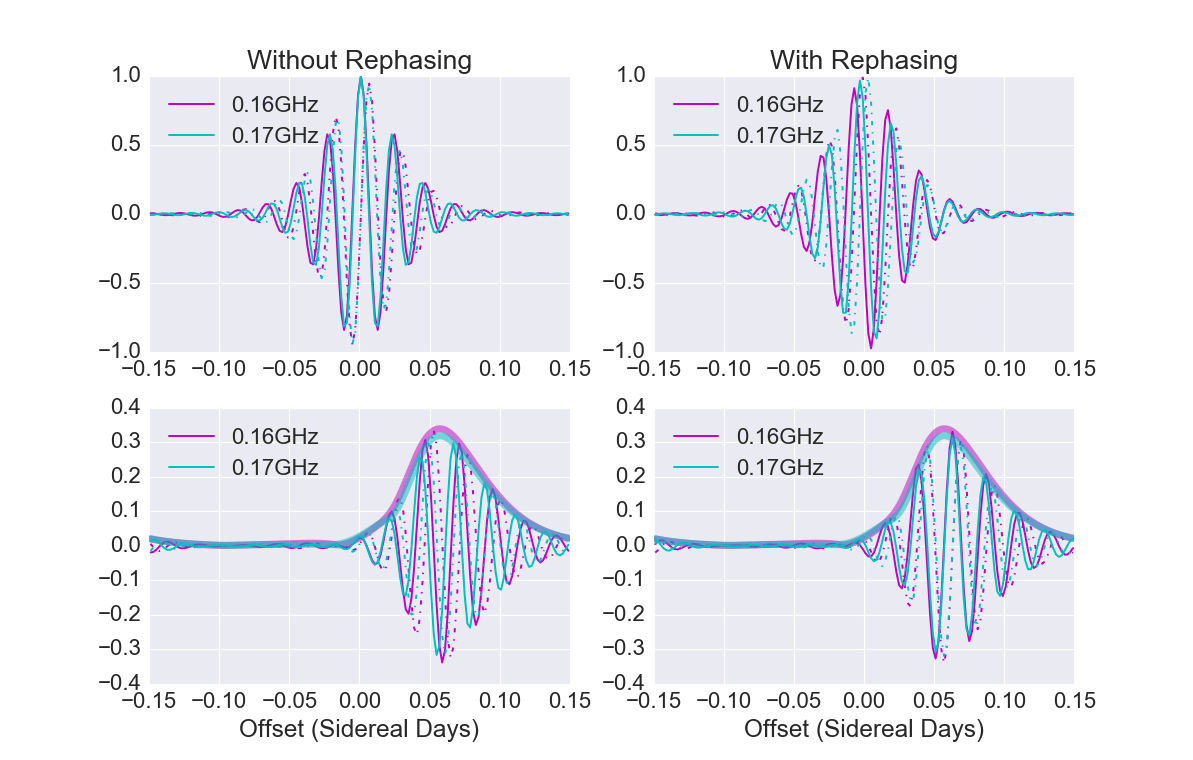
\includegraphics[width=1.1\linewidth]{rephs}
\label{fig:freqdiff}
\caption{Comparisons of the peak phases of two different frequencies. Top panels shows equivalent baselines, bottom shows a pair of near-equivalents. The dot-dashed lines of each color are the imaginary parts, and the solid lines are the real parts. For near-equivalent case, we also draw the magnitude by the broad envelops. }
\end{figure}


\section{Analysis}
\subsection{Numerical Test \label{sec:Techniquet}}

To test the robustness of Eq.(\ref{eq:final}), we need to compare the amplitude and phase of the integral weight $\Theta$ 
for a pair of baselines with products of simulated visibilities of those baselines. For computational simplicity, we shall use a single frequency channel of $150$MHz for the comparison. We may use this simplification without compromising generality because Eq. (\ref{eq:final}) is valid for a range of frequency channels if an only if it's valid for each single channels, provided that different channels are combined with rephasing as desscribed in Sec. \ref{sec:rephs}. 

For the simulation, we take N random realizations of the sky
on a healpix map (\cite{Heal}, \cite{HealPrimer}) \footnote{We use functionalities in the python package AIPY for healpix mapping
as well as coordinate transforms. }. For each realization, each pixel is given a Gaussian random value
of brightness temperature. We then rotate the baseline positions with
the appropriate rotation matrix, recording the visibilities, for each
baseline \footnote{As a caveat, there are two obvious ways to achieve the rotation. One
can either fix the sky and rotate the baselines, or the other way
around. We found however, that we must not physically rotate the sky
map, for the numerical round-offs due to finite resolutions of the
map turns out to be significant. Thus we let the sky, represented
by the healpix map, be fixed, and rotate the baselines. }. The resulting visibilities for the two baselines are then convolved
via the Fourier convolution theorem, to obtain values of the cross
correlation as a function of time-offset. The peak of the curve then
corresponds to maximum redundancy. The accuracy of this result is
limited by (simulated) cosmic variance and finite spacial resolution,
and hence can be beat down by averaging over a large number of universes.
A numerical estimate of the error of the peak height with $N=1$ is
$\lesssim20\%$, and thus with $N=2500,$ we achieve an error of peak
height $<0.5\%$. 

The comparison is show in Fig. \ref{fig:numerics}. 
Since the sensitivity contribution is inferred from height of the peak of the cross-multiplied visibilities as a function of time. 
We first compare the simulation to the analytical weight $\Theta$ for a pair of equivalent baselines, then normalize the peaks 
of the near-equivalent baselines to that of the equivalent ones. 
In Fig. \ref{fig:numerics}  we show on the top comparison of
the convolution of an equivalent baseline of PAPER-128, normalized to 1 at the
peak, whose location is at zero time offset as expected. On the bottom we show
comparison of a near-equivalent baseline pair, of classes sep1,0:1,1 and sep1,1:1,1. The peaks
are normalized with the same factor as the peak height on the top,
i.e. the two plots have thus the same scale on the vertical axis.
The height of the plot thus quantifies the added sensitivity. We see at a peak of around 0.055 sidereal days, or 1.32 hours, the two baselines are maximally redundant. 

\begin{figure}[H]
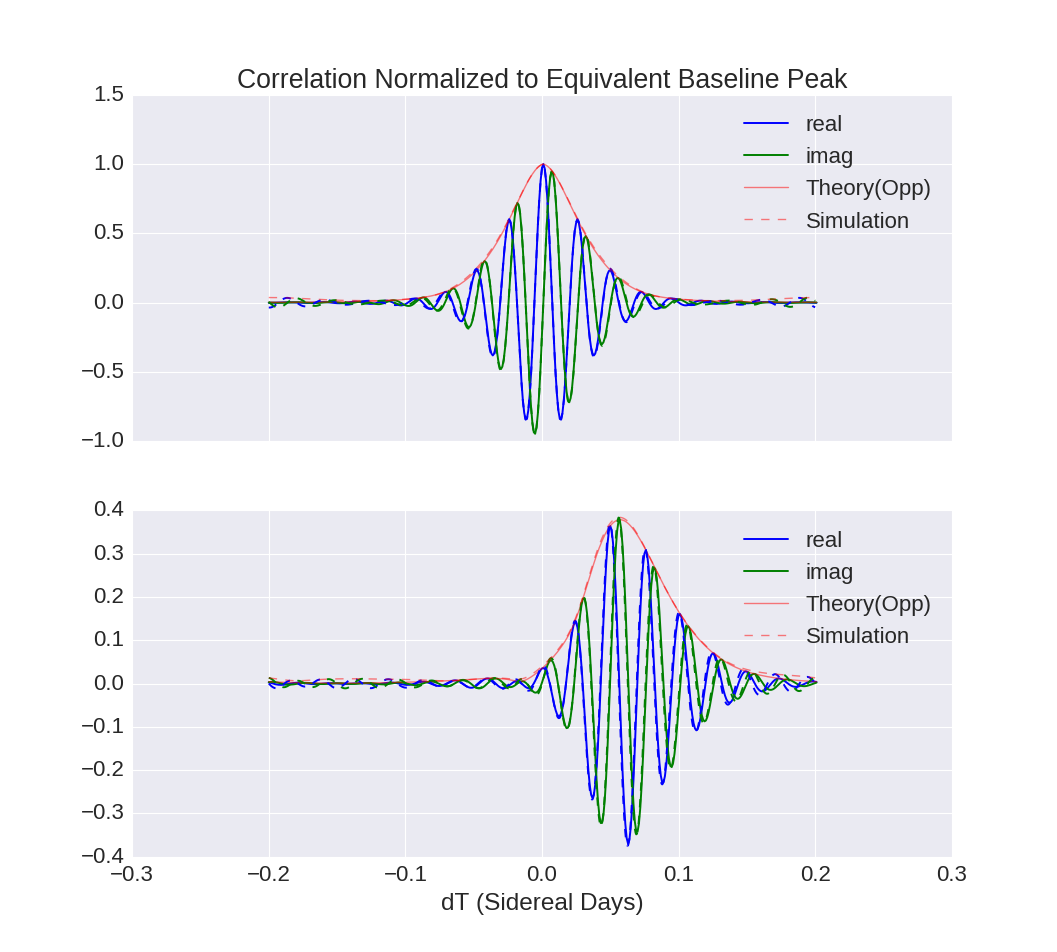
\includegraphics[width=\linewidth]{corr}
\label{fig:numerics}
\caption{Numerical comparisons of the visibility correlation peaks to the $\Omega$ factor in Eq.(\ref{eq:final}). We generated 2400 instances of Gaussian random sky on healpix maps, computed visibilities and cross correlated them to find the correlation.  Top panel shows the equivalent baseline pairs sep1,0 against itselt, bottom show set1,0:1:1.  Evaluations of weight $\Theta$ are shown with solid curves, and the visibility correlations of simulated random sky is given with dashed lines. In both cases blue denotes real part, green the imaginary part, and red the magnitude. We see that in both cases the theory and simulation line up in both amplitude and phase.}
\end{figure}


At the optimal time separation, the integral in Eq. \eqref{eq:final}
is maximized. Thus as another check we expect the two beams to have to same fringe pattern
(frequency and phase). Due to the time delay, however, the beam center
would be slightly shifted with respect to each other. This we show
in Fig. \ref{fig:Beam-fringe-pattern}. The left and middle panels show the beam fringe
patterns for baselines sep2,0 and sep2,1, delayed by 0.0325 sidereal days,
and the right panel shows their cross product. The fringe pattern
indeed cancels out as we expect. 

%\begin{widetext}
\begin{figure}[H]
%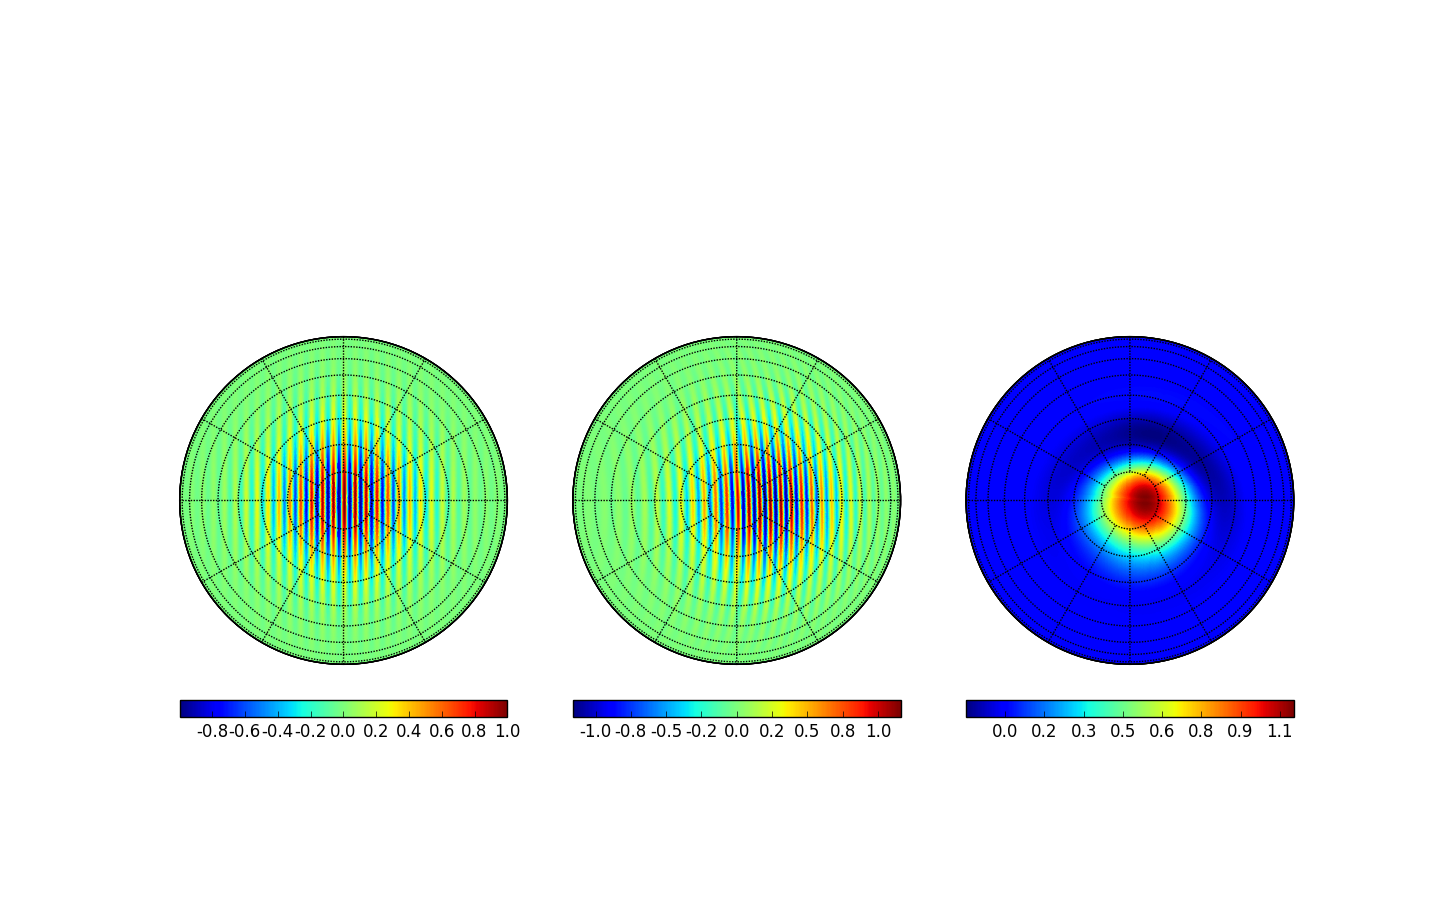
\includegraphics[scale=0.5]{fringe_res}
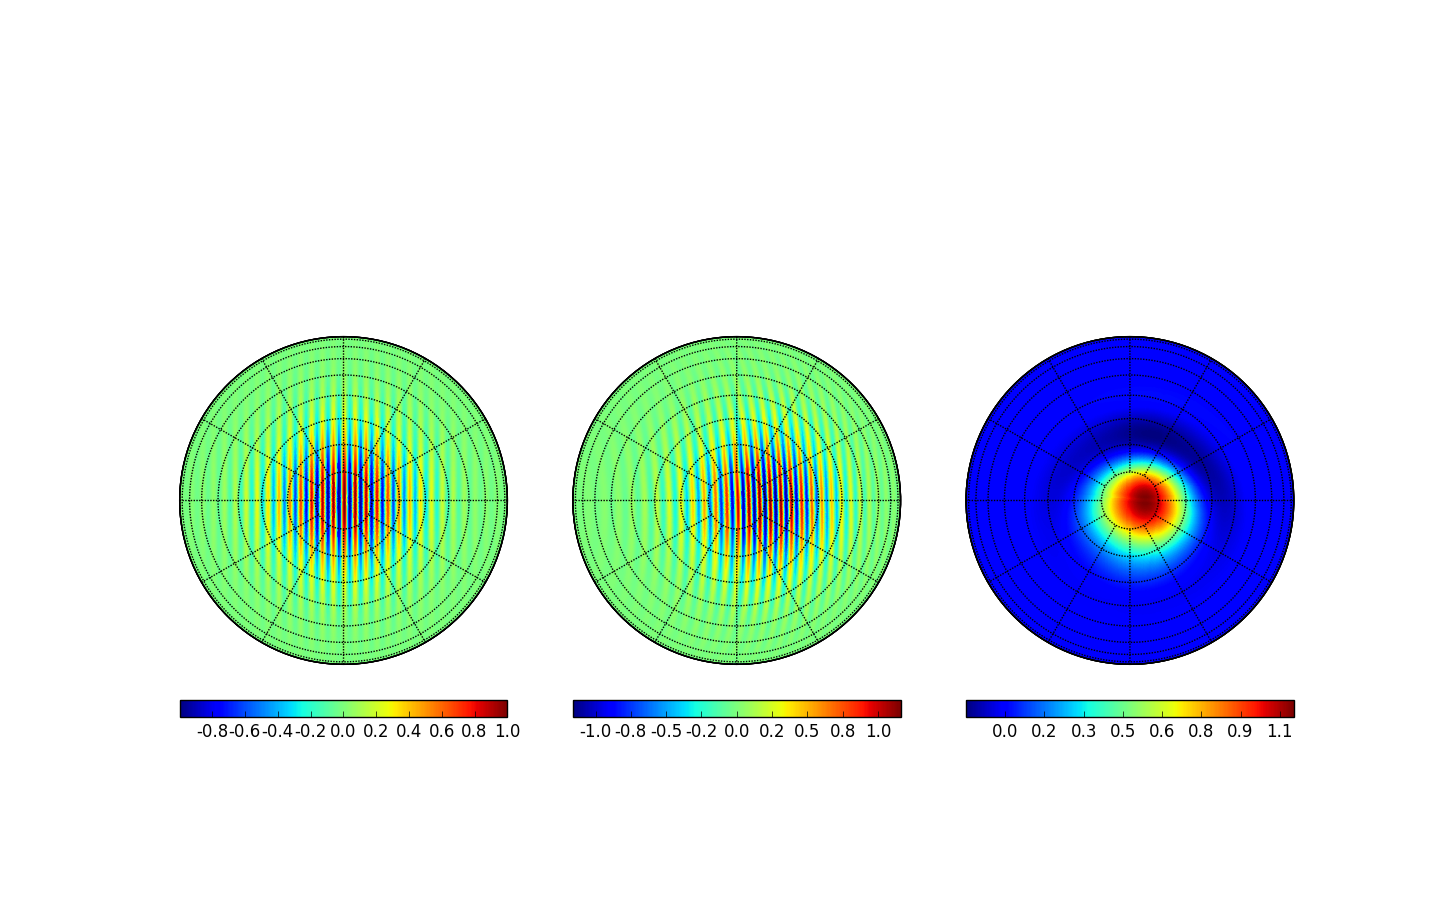
\includegraphics[width=\linewidth]{fringe_res}
\caption{Beam fringe pattern of sep2,0(left), sep2,1 at a time delay (middle),
and their conjugate product. Frequency of $\nu=0.15\text{GHz}$ is
chosen and only the real components are shown. \label{fig:Beam-fringe-pattern}}
\end{figure}
%\end{widetext}


\subsection{Expected Sensitivity Contributions}

Having verified Eq. \eqref{eq:final}, we can thus predict the sensitivity contributions of a
particular baseline pair simply by computing the integral.
Intuitively we expect the sensitivity to depend on both the uv coverage of the baseline and the patch of sky inside the beam. A larger beam like PAPER-beam would tolerate larger time-offsets because more sky area can coincide in the two beams. To keep the flow of the discussion, we shall focus on results of PAPER-128, and present the results for HERA in the Appendix. 
Having computed all of the baseline pairs, we find that baseline pairs that are mirror images of each other 
give the same amount of redundancies (peak height), with the opposite time offset, as expected from symmetry. 
For example, sep1,0:1,1 is mirror image of sep1,0:1,-1 and these two baseline pairs
give the same sensibility contribution. Thus in our results we shall only show a subset of representative baseline pairs 
that give different informations. 

In the top panel of Fig. \eqref{fig:sensplot} below
we show the peak heights and locations for a variety of baseline combinations.
We see that baseline pairs that have crossings at a smaller time delay
tend to have higher correlations. In other words, correlation peaks
that are closer to zero time lag are higher. This is expected since
a) the longer the time delay, the more the antennas have moved with respect
to the sky and hence the less overlaps in patch of sky surveyed, b) smaller optimal
time-offset corresponds to smaller differences in orientation, and hence in length of
baselines in PAPER. 

\begin{widetext}
\begin{figure}[H]
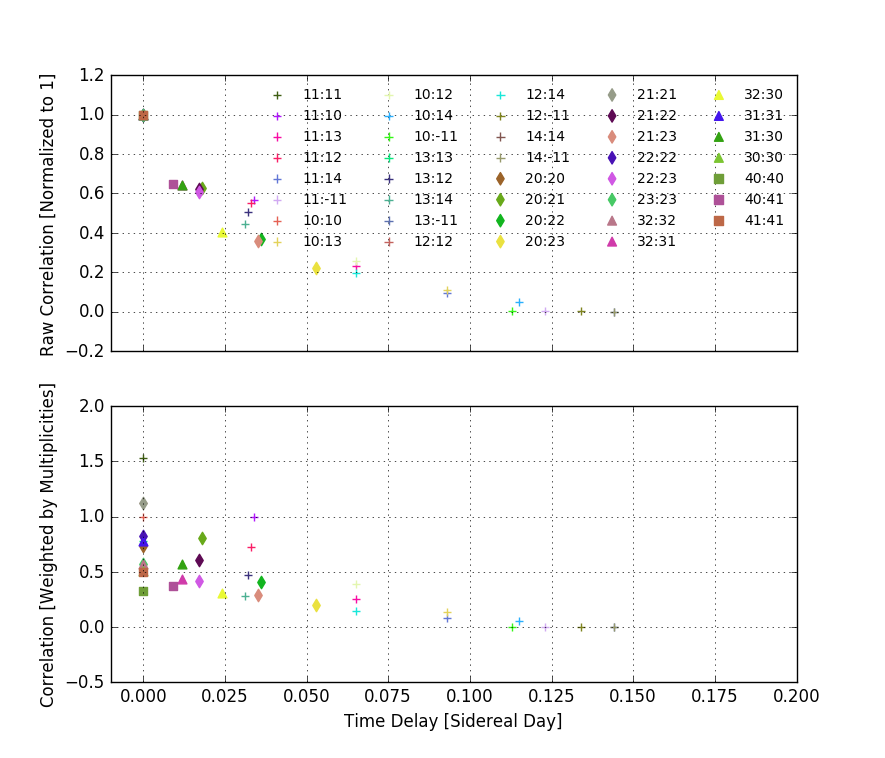
\includegraphics[scale=0.5]{sensitivity}
\label{fig:sensplot}
\caption{Relative sensitivity contributions of selected baseline combinations in PAPER-128. In the legend m,n:p,q denotes cross
multiplying PAPER-128 baselines of east-west, north-south separations (m,n) and (p,q) respectively. The top
panel shows the peak height (degree of correlation) of each baseline
combination, while the bottom panel multiplies the heights by the
corresponding multiplicities as in Eq. \eqref{eq:sensul}, and in some cases an extra factor of $\sqrt{2}$ (explained in text). 
In weighting by the multiplicity (bottom), we have chosen to fix the sensitivity 
contribution of 1,0:1,0 to unity. }
\end{figure}
\end{widetext}

To determine that actual relative contribution to sensitivity of these
baseline pairs, we have to take into account of the multiplicities of
these baselines, or the size of the equivalency classes in a mathematical
language. By these we mean how many physical antenna pairs have the
same length and orientation. Looking at Fig. \ref{fig:sensplot}
we see for example sep1,0 will have higher multiplicity than sep2,0,
or sep1,1. The latest release of PAPER-64 data uses the 128-equivalent baselines sep2,1,
sep2,0 and sep2,-1 \cite{Ali2015}, and achieved a $2\sigma$ upper
limit of $22.4mK^{2}$. There, the three sets of equivalent baselines
are only cross multiplied by itself. Assuming that each baseline delivers
the same quality of data (i.e. they have the same height of correlation
peaks, which is in our normalization equal to unity), the relative
contribution to sensitivity can be estimated. 

First we can average of the visibilities of the equivalent baselines. Since the core of PAPER-128 has 16 by 7 antenna configuration, there
are $M=(16-|m|)\times(7-|n|)$ copies of the baseline sepm,n. This means
that if we add visibility measurements of all these equivalent baselines,
we get a factor of $\sqrt{M}$ reduction in noise
level $\sigma_N$ of the visibility. The sensitivity contribution of sepm,n, cross multiplied with sepm',n'  thus roughly speaking scales as $\sqrt{\left((16-|m|)(7-|n|)(16-|m'|)(7-|n'|)\right)}=\sqrt{MM'}$.
For cross-multiplications of near-equivalent baselines of
types sepm,n and sepm',n', we get a effective weight: 

\begin{equation}
\widetilde{\Theta}_{bb'} \propto \Theta_{bb'}\times\sqrt{MM'}.\label{eq:sensul}
\end{equation}

We are being sloppy here for simplicity. As we derive in Appendix \ref{sec:appB}, this weight should be corrected by a factor proportional to the signal to noise ratio of a single-baseline visibility $\rho_0=\sigma_S^2/\sigma_N^2$:

\begin{equation}
\label{eq:tildereal}
\widetilde{\Theta}_{bb'}=\frac{\Theta_{bb'}\sqrt{M_bM_{b'}}}{\sqrt{1 + \rho_0 \left(M_b+M_{b'} \right)}}.
\end{equation}

Shown in the bottom panel of Fig. \eqref{fig:sensplot} is the peak heights weighted
by the multiplicity factor. Points that have zero time delay are the equivalent baseline pairs and their weighted correlation values simply reflect the multiplicity factor. For clarity of presentation we have "folded over" the negative time delays and combined baseline pairs that are identical modulus parity, 
or in other words are mirror images of each other, by summing over them to get an extra factor of $\sqrt{2}$. For example, 
instead of plotting 1,1:1,1 and 1,-1:1,-1 separately, we plot 1,1:1,1 with twice the multiplicity. Similarly, baseline pairs such as 
1,0:1,1 also get the factor of 2 because they are identical to 1,0:1,-1. Baseline pairs such as 1,0:1,0, or 1,1:1,-1 do not get
the factor of $\sqrt{2}$ because their mirror images are themselves. 




Finally we estimate the power spectrum by inverse covariance weighting:
\begin{equation}
\begin{aligned}
 P(k_{\tau}) &= \frac{\sum_{bb'}P(k_{b,\tau})/\sigma_P^2(bb')}{\sum_{bb'}\sigma_P^2(bb')}, \\
 &= \frac{\sum_{bb'}P(k_{b,\tau})\widetilde{\Theta}_{bb'}^2}{\sum_{bb'}\widetilde{\Theta}_{bb'}^2},
 \end{aligned}
\end{equation}
where the sum is over classes of baseline pairs. 
Thus the total signal to noise ratio is given by
\begin{equation}
\rho \propto \frac{\sum_{bb'}^N\widetilde{\Theta}_{bb'}^2}{\sum_{bb'}^N\widetilde{\Theta}_{bb'}},
\end{equation}


where $N$ is the total classes of baseline pairs used. When all the $\widetilde{\Theta}$ are unity, $\rho$ improves by $1/\sqrt{N}$ scaling. When $\Theta<1$ it's clear that adding more baselines is not always going to lead to improvement. Thus for given antenna array we should restrict antenna pairs with $\widetilde{\Theta}$ above a certain $\widetilde{\Theta}_{min}$ for maximum sensitivity. 


To move forward we must give an estimate of $\rho_0$ in Eq.\ref{eq:tildereal}. 

%\subsection{Notes on Data, Foreground and Noise}
%Unlike the simulated clean EOR signal, real data are dominated by foreground %and thermal noise, neither of which turns out to exhibit the correlation %pattern seen in Fig.  \ref{fig:numerics}. Foreground exhibits long-range %correlations and would lead to high responses at wide range of time-offsets. %Instrumental noise for different baselines/antenna-pairs, on the other hand, are uncorrelated and thus exhibit responses consistent with zero at all time offsets. 
%To illustrate, we use the second observing season of PAPER-128 data, taken from Jan. 21st to March 7th of 2014. To illustrate the effect of noise and foreground, we use the data before fringe-rate and delay filtering. 

\section{Conclusion}
Redundant arrays are designed to maximize sensitivity. Current generations of redundant radio arrays, such as those probing the power spectrum of the epoch of reionization could benefit from data analysis techniques that improve the sensitivity. We present an intuitive analysis of cross-multiplying baselines that are close in length and orientation to each other. Given an antenna array configuration, our method quickly identifies the best baseline pairs to cross-multiply and predict the expected sensitivity contribution. With the predicted result one can improve existing power-spectrum pipelines through 3 simple steps. 1). Rephase the visibilities prior to delay transforming by the zenith displacement (or more accurately by the phase predicted by our numerical analysis). 2). Shift the visibilities in time. 3) Cross multiply the visibilities of the two baselines  to form the power-spectrum. 4) Finally combine the different baseline pairs by appropriate inverse-covariance weighting that takes into account the predicted sensitivity contributions of each case. 

\appendix
\section{\\Hera Analysis}
\begin{widetext}
\begin{figure}[H]
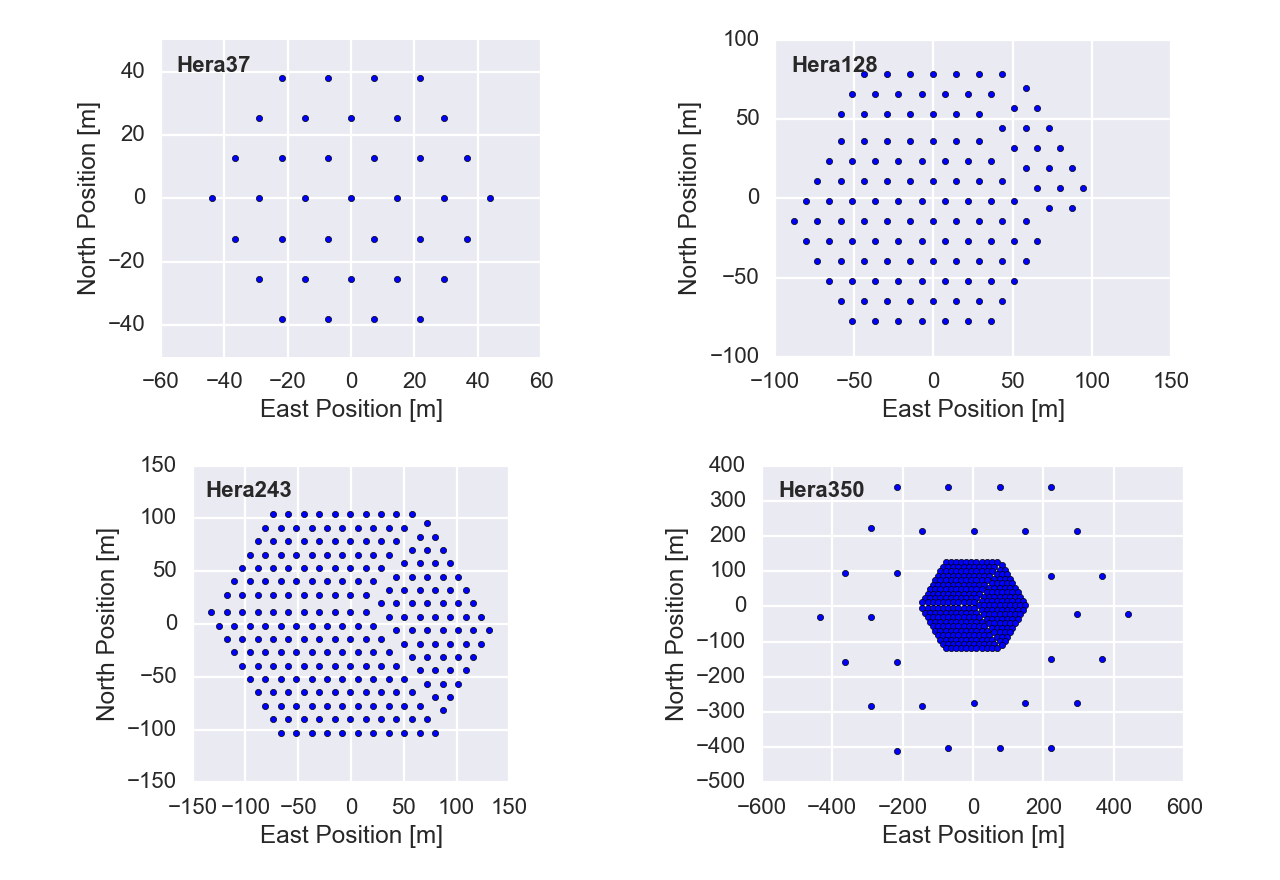
\includegraphics[scale=0.55]{HeraAntpos}

\caption{Planned Hydrogen Epoch of Reionization Array antenna configurations. For HERA350, only the 320 elements in the core are shown. \label{fig:HeraAntpos}}
\end{figure}
\end{widetext}

\section{\\Derivation of Noise Covariance \label{sec:appB}}

Now to be a little more careful about the scaling relations above, we combine the different power spectrum measurements by inverse covariance weighting \footnote{In practice techniques such as bootstrapping is often used, see for example \citep{Ali2015}}. We shall separate the visibility and power spectrum into signal and noise contributions:
\begin{equation}
\begin{aligned}
V &= V_S+V_N,\\
P &= P_S+P_N.
\end{aligned}
\end{equation}
We shall denote the noise covariance of power spectrum and visibility
\begin{equation}
\begin{aligned}
\sigma_V^2 &= \langle |V_N|^2 \rangle,\\
\sigma_P^2 &= \langle P_N^2 \rangle.
\end{aligned}
\end{equation}
One may notice that we have used a single covariance for the complex quantity visibility. It's simple to show that the same result holds if we use a separate real and imaginary components, as long as they are independent of each other. In fact, for simplicity and without loss of generality we shall treat the visibility as a real quantity in the rest of this derivation. 
Note that though we can assume $\langle V_N^{odd-power}\rangle=0$, the same is not true for $P_N$. 

Then the variance of $P$ constructed with visibilities $V_1$ and $V_2$ from two baseline classes can be estimated\footnote{We assume all noise terms to be independent for simplicity, in practice the correlation of different measurements ifrom equivalent baselines are alleviated by grouping the baselines in the class and the days of observation, as in \cite{Ali2015}}:
\begin{equation}
\begin{aligned}
\sigma_P^2 &= \langle P^2\rangle -\langle P \rangle^2,\\
&\propto \langle \frac{(V_{1S}+V_{1N})^2 (V_{2S}+V_{2N})^2}{\Theta^2} \rangle - \langle \frac{(V_{1S}+V_{1N}) (V_{2S}+V_{2N})}{\Theta} \rangle ^2,\\
&= \frac{1}{\Theta^2} \left( V_{1S}^2\sigma_{V2}^2+V_{2S}^2\sigma_{V1}^2+\langle V_{1N}^2 V_{2N}^2\rangle\right), \\
&= \frac{1}{\Theta^2} \left[ V_{S}^2(\sigma_{V2}^2+\sigma_{V1}^2) + \sigma_{V1}^2 \sigma_{V2}^2\right], 
\end{aligned}
\end{equation}

where in the second last line we have substituted visibility noise covariance. In the final line we used Wick's theorem and the fact that the signal from two visibilities are equal. 

Recall from the discussion on multiplicities we can write
\begin{equation}
\sigma_V^2=\frac{\sigma_0^2}{M},
\end{equation}
where $\sigma_0$ is some single-baseline noise level. Letting $\rho_0=V_S^2/\sigma_0^2$ be the signal to noise ratio for a single baseline, we can write

\begin{equation}
\begin{aligned}
\sigma_P^2 & \propto  \frac{\sigma_0^4}{\Theta^2} \left[ \rho_0 \left(\frac{1}{M_1}+\frac{1}{M_2} \right) + \frac{1}{M_1 M_2}\right], \\
&\propto \frac{1}{\widetilde{\Theta}_{12}^2},
\end{aligned}
\end{equation}
where we have defined a slightly modified version of the effective weight (compare with Eq. \ref{eq:sensul}):
\begin{equation}
\widetilde{\Theta}_{12}=\frac{\Theta_{12}\sqrt{M_1M_{2}}}{\sqrt{1 + \rho_0 \left(M_1+M_{2} \right)}}.
\end{equation}
\bibliographystyle{apj}
%\nocite{*}
\bibliography{draft_working}

\end{document}
